\scanpage{571}
\mspage{290}

more closely the congruential modular varieties
$M_{1,1}[3]$ and $M_{1,1}[5]$, corresponding to
``geometric'' modular groups:
\[
\unsure{(}\quad
\left\{
\begin{array}{l}
S\Gamma'_3 = \underbrace{\mathrm{Sl}(2,\mathbb F_3)}_{\substack{\text{order }4.3.2\\=24}}/\mathord{\pm}1
\quad \text{of order }12\;\underset{\unsure{\deleted{\unsure{\infty}}}}{\phantom{a}}
\subset \underbrace{\mathrm{GP}(1,\mathbb F_3)}_{\text{order }24}\simeq\mathfrak S_4
\\[1.5em]
\unsure{\inserted{\text{in fact, we must have } S\Gamma'_4\simeq A_4}}
\\[1.5em]
S\Gamma'_5 = \underbrace{\mathrm{Sl}(2,\mathbb F_5)}_{\substack{\text{order }6.5.4\\=120}}/\mathord{\pm}1
\quad \text{of order }60
\subset \underbrace{\mathrm{GP}(1,\mathbb F_5)}_{\text{order }120}\simeq\text{group of the \uline{bi}icosahedron}
\end{array}
\right.
\tag{74}
\]

Unless I am mistaken, these groups \unsure{are|\deleted{are}} \inserted{resp.} the groups $A_4$ of the
oriented \uline{tetrahedron}, and the one $A_5$ of the oriented icosahedron.
If I remember rightly, the cases
$n=2,3,4,5$ exhaust the cases of congruential modular \deleted{\unsure{varieties}}\inserted{curves}
$M_{1,1}[n]$ which are \uline{rational}
-- it is a remarkable thing that through them one finds
all the regular \inserted{finite} polyhedra \unsure{with} triangles for faces
\margin{except one, with ``folded-back edges'' -- the one in figure (76), cf. below\ldots}
-- it was clear \inserted{\unsure{a priori|a-priori}}, from the \unsure{isomorphism|isomorphism} between
$\mathcal T'_{1,1}$ and the ``triangula- oriented cartographic group'' $\pi'_{0,3}$,
that we should find again all
the finite regular polyhedra \unsure{with|\deleted{tri}} triangles for faces
in this way, but not that
this should be with \unsure{congruence|congruences} subgroups,
very precisely. The table obtained is
then the following

\scanpage{572}

\[
\begin{array}{lll}
\text{group }G=S\Gamma'_n & \text{modular curve} & \text{type of regular oriented polyhedron}\\[.5em]
\left\{\begin{array}{l}D_3\simeq\mathfrak S_3\\ A_4\\ \mathfrak S_4\\ A_5\end{array}\right.
&\begin{array}{l}M_{1,1}[2]'\\M_{1,1}[3]\\M_{1,1}[4]\\M_{1,1}[5]\end{array}
&\begin{array}{l}\text{spherical bitriangle}\\\text{tetrahedron}\\\text{octahedron}\\\text{icosahedron}\end{array}
\end{array}
\tag{75}
\]

As other rational modular curves (not congruential)
Galois over $\widetilde M_{1,1}$, there would still be
the quotients of the preceding ones by
invariant subgroups of the $S\Gamma'_n$, distinct from the whole group and from $1$.
One finds as possible quotients

\noindent a) Case $\mathfrak S_3$; the quotient $\pm1$ (via the sign)

\noindent b) Case $A_4$: the quotient $\mathbb Z/3\mathbb Z=C_3$
(via $\mathfrak S_4\to\mathfrak S_3$, inducing $A_4\to C_3$)

\noindent c) Case $\mathfrak S_4$: the quotient $\mathfrak S_3$, and the quotient $\{\pm1\}$ of the latter.

(For d), there is nothing, $A_5$ being a simple group)

\deleted{\unsure{The varieties}}

The rational modular curves obtained \unsure{are}
reduced to the two cases a) and b) (which are
\unsure{found again|found again} in c)). In case a), one finds
the \inserted{quadratic} covering of $Y=\mathbb P^1(\mathbb C)-\{0,1,\infty\}$, which is
unramified at $\infty$ (for the ramification index must
divide $2$ and $3$), which therefore corresponds to the covering
\[
\deleted{\unsure{\sqrt{x(x+1)}}}\qquad y=\sqrt{x(x-1)}
\]
and to the regular spherical map of type $(2,1)$
(vertices of index $2$, faces of index $1$)
\figure{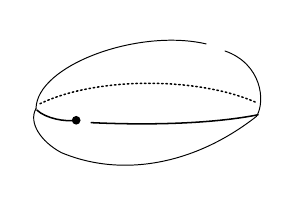
\begin{tikzpicture}[x=1cm,y=1cm,baseline=-0.35ex]
\draw[line width=0.35pt,line cap=round]
(-1.40,0) .. controls (-1.39,0.55) and (-0.10,1.02) .. (0.76,0.82);
\draw[line width=0.35pt,line cap=round]
(1.00,0.73) .. controls (1.46,0.57) and (1.52,0.10) .. (1.40,-0.10)
.. controls (0.61,-0.72) and (-0.32,-0.88) .. (-1.08,-0.56)
.. controls (-1.34,-0.42) and (-1.50,-0.18) .. (-1.40,0);
\draw[densely dotted,line width=0.55pt,line cap=round]
(-1.35,0.06) .. controls (-0.62,0.41) and (0.68,0.40) .. (1.41,0.07);
\draw[line width=0.55pt,line cap=round]
(-1.39,-0.02) .. controls (-1.27,-0.13) and (-1.03,-0.17) .. (-0.90,-0.15);
\fill (-0.89,-0.15) circle[radius=0.055];
\draw[line width=0.55pt,line cap=round]
(-0.70,-0.18) .. controls (0.17,-0.22) and (0.91,-0.18) .. (1.42,-0.08);
\end{tikzpicture}}
\unsure{formed|formed} of one vertex, \unsure{on} an edge (equator) bounding two faces which are monogons.

Case b) is the cyclic covering of order $3$:
ramified only at $0$ and at $\infty$ (at $1$ the ramification index must be a divisor of $2$ and of $3$,
hence is $1$) hence regular spherical map of

\scanpage{573}
\mspage{291}

type $(3,3)$, with edges which are loops
\deleted{\illegible{1}}\inserted{folded back}

(76) \figure{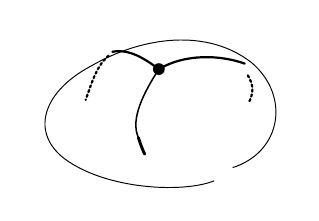
\begin{tikzpicture}[x=1cm,y=1cm,baseline=-0.35ex]
\draw[line width=0.35pt,line cap=round]
(0.89,-0.66) .. controls (1.51,-0.46) and (1.62,0.25) .. (1.13,0.67)
.. controls (0.57,1.11) and (-0.25,1.01) .. (-0.91,0.63)
.. controls (-1.57,0.28) and (-1.71,-0.29) .. (-1.14,-0.62)
.. controls (-0.61,-0.94) and (0.27,-0.98) .. (0.65,-0.83);
\draw[line width=0.8pt,line cap=round]
(-0.05,0.59) .. controls (-0.23,0.72) and (-0.42,0.85) .. (-0.64,0.81);
\draw[densely dotted,line width=0.8pt,line cap=round]
(-0.69,0.76) .. controls (-0.86,0.61) and (-0.91,0.38) .. (-0.98,0.20);
\draw[line width=0.8pt,line cap=round]
(-0.05,0.59) .. controls (0.29,0.79) and (0.73,0.77) .. (1.04,0.66);
\draw[densely dotted,line width=0.8pt,line cap=round]
(1.08,0.51) .. controls (1.16,0.38) and (1.15,0.28) .. (1.09,0.16);
\draw[line width=0.55pt,line cap=round]
(-0.05,0.59) .. controls (-0.23,0.31) and (-0.42,-0.04) .. (-0.31,-0.28);
\draw[line width=1.05pt,line cap=round]
(-0.31,-0.28) .. controls (-0.29,-0.35) and (-0.25,-0.45) .. (-0.23,-0.49);
\fill (-0.05,0.59) circle[radius=0.075];
\end{tikzpicture}}
: $1$ single vertex,
three folded-back edges coming out of it, one
triangular face. [These modular varieties are
too close to $\widetilde M_{1,1}$ -- with an automorphism
group (quotient of $\Gamma'_\infty=\mathrm{Sl}(2,\unsure{Z|\mathbb Z})$) too small,
to be able to be rigidifying (the Galois-Poincaré group of the covering
would have to
be a multiple of $12$\inserted{(multiple of $4$ and of $6$ ?!)}, for \deleted{\illegible{1}} the modular curve to have a chance of being rigidifying. These
cases thus seem distinctly less interesting.

There would be reason moreover, in each of the
three remaining cases of (75) (thus setting aside the
first case, which corresponds to $M_{1,1}[2]'$ and is
more or less understood), to make explicit the relation
between the points of the corresponding rational curves,
and between \inserted{elliptic curves with} Jacobi rigidifications,
of level $3,4,5$ respectively. And there
are surely precise things in Klein,
but one would like to do things a little
finer, which are valid simultaneously
in \unsure{all characteristics|every characteristic} i.e. over general
base schemes. This concern seems intimately linked to the question of the operations of
$\Gamma_{\mathbb Q}$ on the isomorphism classes of maps, and

\scanpage{574}

more particularly of regular
spherical maps. It is quite extraordinary that
Jean Malgoire, in the three years that the
question has been there, has not yet touched it
-- God knows it is juicy!

Supplement on the cross-ratio.

Let $x_1,x_2,x_3,x_4$ be \deleted{variables, \unsure{at|or} $\infty$}\inserted{sections \inserted{\unsure{everywhere}} distinct} of
$\mathbb P^1_S$, we want to construct the \unsure{corresponding} section $\lambda$
of $\unsure{U|\mathbb U}_{0,3}=\mathbb P^1_S-\{0,1,\infty\}_S$.
Let $a,b,c,d$ be sections
(local) of $\mathcal O_S$, \inserted{with \deleted{\illegible{1}} $ad-bc$ invertible,} such that
\[
u=u_{a,b,c,d}:\quad z\longmapsto\frac{az+b}{cz+d}
\tag{77}
\]
transforms $(x_1,x_2,x_3)$ into $(0,1,\infty)$ -- we
shall therefore have
\[
\lambda=u(x_4).
\tag{78}
\]
The conditions on \unsure{$\xi$|\deleted{\illegible{1}}} $(a,b,c,d)$ for $ux_1=0$ etc. are
\[
\left\{\begin{aligned}
ax_1+b&=0\\
ax_2+b&=cx_2+d\\
cx_3+d&=0
\end{aligned}\right.
\]
which give, if for example $a$ is invertible (otherwise, we
can assume $\unsure{c}$ invertible\ldots) on solving for $b,c,d$
\[
\left\{\begin{aligned}
b&=-ax_1\\
cx_2+d&=a(x_2-x_1)\\
cx_3+d&=0
\end{aligned}\right.
\qquad\left|\begin{aligned}
c&=a\frac{x_2-x_1}{x_2-x_3}\\
d&=-a\frac{x_2-x_1}{x_2-x_3}x_3
\end{aligned}\right.
\]
whence
\[
\lambda=\frac{ax_4+b}{cx_4+d}
=\frac{a(x_4-x_1)}{a\frac{x_2-x_1}{x_2-x_3}x_4-a\frac{x_2-x_1}{x_2-x_3}x_3}
=\frac{(x_4-x_1)(x_2-x_3)}{(x_2-x_1)(x_4-x_3)}
\]

\scanpage{575}
\mspage{292}

\[
\lambda(x_1,x_2,x_3,x_4)=\frac{(x_4-x_1)(x_2-x_3)}{(x_2-x_1)(x_4-x_3)}
\tag{79}
\]

As a rational function in $x_1,x_2,x_3,x_4$,
(with coefficients in a fixed integral domain) it
is characterized by the two properties: a) invariance \unsure{with respect} to a (same)
homographic transformation on the variables, \inserted{$x_1,x_2,x_3,x_4$,} \deleted{and}
\[
f(ux_1,ux_2,ux_3,ux_4)=f(x_1,x_2,x_3,x_4),
\]
\inserted{and} b)
\[
f(0,1,\infty,x_4)=x_4
\]
(with a grain of salt to give a
meaning to the first \unsure{side.} We have moreover
c) a remarkable symmetry property,
which we \deleted{\illegible{1}} make explicit by defining a homomorphism
from $\mathfrak S_4$ into the homographic group
(\unsure{morally|normally}, $\mathrm{GP}(1)$)
\deleted{\illegible{1}}
\diagram{
\begin{tikzcd}[ampersand replacement=\&,column sep=large,row sep=large]
\mathfrak S_4 \arrow[rr,"\sigma\mapsto\varphi_\sigma"] \arrow[dr,"\text{epimorphism}","\substack{\text{\unsure{factoring}}\\\text{through}}"'] \&\& \mathrm{GP}(1) \\
\& \mathfrak S_3 \arrow[ur] \&
\end{tikzcd}
}
in such a way that we have
\[
\lambda(x_{\sigma^{-1}1},x_{\sigma^{-1}2},x_{\sigma^{-1}3},x_{\sigma^{-1}4})
=\varphi_\sigma(\lambda(x_1,x_2,x_3,x_4))
\tag{80}
\]
\ldots
